\appendix
\chapter{Energy storage potential and efficiency}
\label{app}
\chaptermark{Energy storage potential and efficiency}

\section*{Energy storage}

We have presented a controller that can leverage energy stored in the rotation of the wind turbine rotors as well as the wind flow field. To get a sense of the relative energy storage capacity of these two mechanisms, the energy stored in the rotation of one turbine operating at the maximum power point is compared to the additional energy available in the flow field to a downstream turbine if the turbine is turned off. At the maximum power point, with optimal tip speed ratio $\lambda_* = \omega R / U_\infty$, the energy stored in the rotation of the rotor is
\begin{equation}
E_\text{rot} = \frac{1}{2} J \omega^2 =  \frac{1}{2} J \left( \frac{\lambda_* U_\infty}{R} \right)^2 ,
\end{equation}
where $J$ is the moment of inertia of the turbine rotor, $\omega$ is the rotational speed of the rotor, $U_\infty$ is the inflow velocity, and $R$ is the radius of the rotor swept area. For a turbine turned off, the energy stored in the wind flow field is equal to the additional power that can be generated by the downstream turbine $P_\text{add}$ times the advective time between the turbines $t_\text{adv}$
\begin{equation}
E_\text{wake} = P_\text{add} \, t_\text{adv}.
\end{equation}
Using the Jensen model~\cite{Jensen1983a}, the additional power is
\begin{equation}
P_\text{add} = \frac{1}{2} \rho \pi R^2 C_P \left[ U_\infty^3 - \left(U_\infty - \frac{2U_\infty a}{(1 + 2ks_x)^2}\right)^3 \right]
\end{equation}
where $C_P$ is the power coefficient, $a$ is the induction factor, $k$ is the wake expansion coefficient, and $2s_xR$ is the spacing between the turbines. The advective time is
\begin{equation}
t_\text{adv} = \frac{2 s_x R}{U_\infty}.
\end{equation}

The ratio of the energy stored in the flow field to the stored rotational energy is therefore
\begin{equation}
\frac{E_\text{wake}}{E_\text{rot}} = \frac{2 \rho \pi R^5s _x}{J} \frac{C_P}{\lambda_*^2} \left[ 1 - \left(1 - \frac{2 a}{(1 + 2ks_x)^2}\right)^3\right]
\end{equation}
If we consider a NREL 5MW turbine~\cite{Jonkman2009a}, with $U_\infty = 8$ m/s, $J = 4.0469\times 10^7$ kg m$^2$, $\lambda_* = 7.75$, $a = 0.292$, $C_P = 0.529$, $R = 63$ m, $\rho = 1.225$ kg/m$^3$, $k = 0.05$, and a streamwise spacing of $s_x = 7$, the rotational energy stored is $E_\text{rot} = 19.6$ MJ (5.5 kWh) and energy stored in the flow field is $E_\text{wake} = 112.2$ MJ (31.1 kWh). The corresponding ratio is
\begin{equation}
\left(\frac{E_\text{wake}}{E_\text{rot}}\right)_\text{NREL} = 5.725,
\end{equation}
which means that in this case the energy that can be stored in the flow is 5--6 times larger than the energy that can be stored in the rotation of the rotor. However, the ratio will depend on the configuration of the farm and will change for larger farms with more wake interactions.

\section*{Storage efficiency}
We have demonstrated that a wind farm can store energy in the flow field by reducing the power generation of upstream turbines. This effectively trades generation between time periods. To estimate the round trip storage efficiency of the wind farm, we simulate the effect of dynamically turning the first row of turbines in the wind farm discussed in Chapter~\ref{subsec:methods-les-farm} on and off, as shown in Figure~\ref{fig:app-dyn}.

\begin{figure}[h!]
\centering
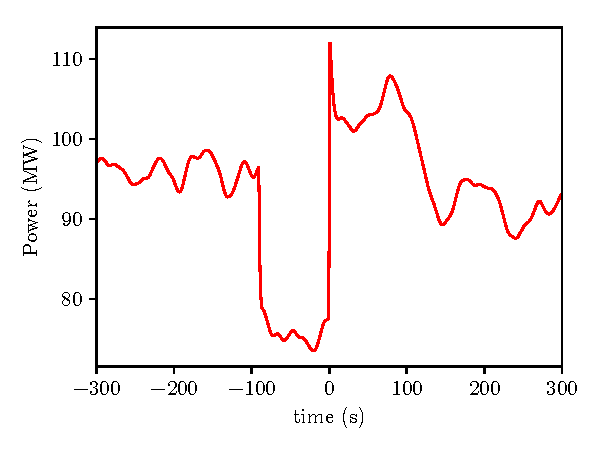
\includegraphics{./fig/fr.pdf}
\caption{Power generation of wind farm, where the first row of turbines is turned off at $t= -90$ s and turned back on at $t=0$ s. }
\label{fig:app-dyn}
\end{figure}

Initially, all turbines are operating at $C_T' = 4/3$, generating approximately 96 MW. At $t=-90$ s, the first row of turbines are turned off, $C_T' = 0$, reducing the generation to approximately 76 MW and eliminating the wake behind the first row of turbines. After 90 seconds, which is the advective time between the turbine rows, the wake from the first row is no longer affecting the generation of the second row. At this point, the first row of turbines is turned back on, which increases the generation to approximately 104 MW. This increased generation continues until around $t = 90$~s, at which point the generation returns to approximately 96 MW. This experiment demonstrates that time-shifting through energy storage in the flow field is feasible. In this case, the storage efficiency was around 45\%; however, the actual efficiency will depend on the turbulent inflow, layout of the farm control actions, and atmospheric conditions.

